\newcommand{\drawSubAutomata}[3]{
  \draw (#1 - 0.7, #2) circle (5pt);
  \node at (#1, #2) {#3};
  \draw (#1 + 0.7, #2) circle (5pt);
  \draw (#1 + 0.7, #2) circle (4pt);
  \draw (#1 - 1, #2 - 0.4) rectangle (#1 + 1, #2 + 0.4);
}

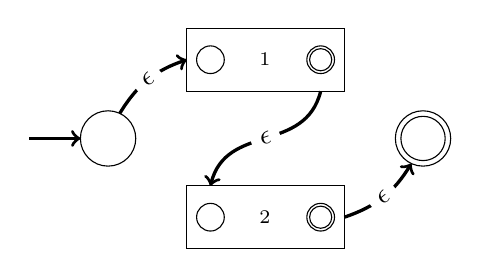
\begin{tikzpicture}[
  vertex/.style = {
    shape = circle,
    draw = black,
    minimum size = 20pt,
    inner sep = 0pt,
    outer sep = 0pt,
  }
]
  \node[vertex] (v1) at (2, 0) {};
  \node[vertex] (v2) at (6, 0) {};

  \draw (6, 0) circle (8pt);  

  \drawSubAutomata{4}{1}{\(\Lang_{1}\)};
  \drawSubAutomata{4}{-1}{\(\Lang_{2}\)};

  \begin{scope}[every path/.style = { very thick, -> }]
    \draw (1, 0) -- (v1);
    \draw (v1) edge[bend left = 20]
      node[midway, sloped, fill = white] {\(\epsilon\)} (3, 1);

    \draw
      (4.7, 0.6) .. controls (4.5, -0.2) and (3.5, 0.2) .. (3.3, -0.6)
      node[midway, sloped, fill = white] {\(\epsilon\)};
    
    \draw[-] (5, -1) edge[bend right = 20]
      node[midway, sloped, fill = white] {\(\epsilon\)} (v2);
  \end{scope}
\end{tikzpicture}
